\chapter{Lucha de Piso}

La lucha de piso es un aspecto emocionante y esencial en la formación de jóvenes artistas marciales. A menudo subestimada, esta disciplina desempeña un papel crucial en el desarrollo de habilidades fundamentales tanto en la defensa personal como en los deportes de combate. En este capítulo, nos sumergiremos en el apasionante mundo de la lucha de piso, adaptándola a un nivel escolar y destinada a jóvenes menores de 18 años.

Desde las técnicas básicas de caída y control hasta las maniobras de sumisión más simples, aquí aprenderemos los fundamentos que sientan las bases para un crecimiento sólido en las artes marciales. Además de las habilidades técnicas, exploraremos la importancia de la disciplina, el respeto y la autoconfianza que la lucha de piso puede inculcar en nuestros jóvenes practicantes.

Descubriremos cómo la lucha de piso se adapta de manera segura y efectiva al entorno escolar, promoviendo valores como la cooperación, el trabajo en equipo y el autocontrol. Aprenderemos cómo estas habilidades pueden ser aplicadas en situaciones de la vida cotidiana y cómo el entrenamiento constante fomenta el respeto por sí mismo y por los demás.

Este capítulo está diseñado para empoderar a nuestros jóvenes practicantes y ayudarlos a desarrollar habilidades físicas y mentales esenciales. Preparaos para embarcaros en un emocionante viaje de autodescubrimiento y crecimiento a través de la lucha de piso, brindando a nuestros jóvenes las herramientas necesarias para enfrentar los desafíos de la vida con confianza y determinación.

¡Comencemos nuestro viaje en el apasionante mundo de la lucha de piso adaptada a jóvenes menores de 18 años!

\section{Preámbulo}

En esta sección, exploraremos los fundamentos esenciales de la lucha de piso y lo que necesitas para comenzar. La lucha de piso es una disciplina emocionante que requiere una preparación adecuada y un conjunto específico de elementos para practicar de manera segura y efectiva.

\begin{itemize}
	\item \textbf{Piso Apropiado:} Un piso adecuado es fundamental para la práctica segura de la lucha de piso. Se recomienda utilizar tatamis o superficies acolchadas que ayuden a absorber el impacto de las caídas y minimicen el riesgo de lesiones. Asegúrate de que el área de entrenamiento esté libre de objetos afilados o peligrosos.

	\item \textbf{Ropa Apropiada:} La elección de la ropa es importante para garantizar la comodidad y la seguridad durante la lucha de piso. Se recomienda el uso de un uniforme de artes marciales adecuado, que suele consistir en un gi (chaqueta y pantalones) y un cinturón para atar la chaqueta. Además, se deben llevar ropa interior adecuada y asegurarse de que el uniforme esté limpio y en buenas condiciones.

	\item \textbf{Jueces y Supervisión:} En la lucha de piso, es esencial contar con jueces o supervisores que puedan observar y evaluar las técnicas y el comportamiento de los participantes. Los jueces deben estar capacitados para hacer cumplir las reglas y garantizar que se mantenga un ambiente seguro y respetuoso durante la práctica o la competición.

	\item \textbf{Normas y Reglas:} Es importante establecer normas y reglas claras para la lucha de piso, que definan qué técnicas son permitidas y cuáles no, así como las pautas de conducta esperadas de los participantes. Las reglas pueden variar según el estilo o la organización, por lo que es fundamental conocerlas y seguirlas en todo momento.

	\item \textbf{Socios de Entrenamiento:} En la lucha de piso, es común practicar con socios de entrenamiento. Selecciona a tus socios con cuidado y asegúrate de que estén igualmente comprometidos con la seguridad y el respeto mutuo. La comunicación con tus socios es fundamental para garantizar una práctica efectiva y segura.

	\item \textbf{Equipo de Protección (Opcional):} Aunque no es siempre obligatorio, el uso de equipo de protección como protectores bucales y protectores de oídos puede ayudar a prevenir lesiones menores durante la lucha de piso. Considera su uso, especialmente en entrenamientos más intensos.
\end{itemize}

\section{Objetivos}

La lucha de piso es una disciplina marcial que va más allá de la fuerza bruta y la agresión. Requiere habilidades técnicas, resistencia física y mental, así como una comprensión profunda de la estrategia. En este capítulo, exploraremos los objetivos fundamentales de la lucha de piso, con un énfasis especial en el desarrollo del control, y cómo esta disciplina puede enriquecer tu viaje en las artes marciales.

\begin{itemize}
	\item \textbf{Desarrollo de Técnicas de Control:} El objetivo principal de la lucha de piso es aprender a controlar y someter a un oponente en el suelo. Esto incluye el dominio de técnicas de inmovilización y sumisión, donde el control es esencial.

	\item \textbf{Mejora de la Resistencia Física:} La lucha de piso requiere una gran resistencia física para mantener el control durante los combates prolongados. El entrenamiento constante contribuye al desarrollo de la resistencia cardiovascular, la fuerza muscular y la agilidad.

	\item \textbf{Fomento de la Autodisciplina:} El control sobre uno mismo y la autodisciplina son fundamentales en la lucha de piso. Los practicantes aprenden a mantener la calma y tomar decisiones estratégicas incluso en situaciones de alta presión.

	\item \textbf{Desarrollo de la Conciencia Corporal:} Entender la posición y movimiento del propio cuerpo es esencial en la lucha de piso, especialmente para mantener el control sobre el oponente. Esto se traduce en una mayor conciencia corporal y coordinación.

	\item \textbf{Mejora de la Toma de Decisiones:} La lucha de piso implica tomar decisiones rápidas y efectivas en tiempo real, especialmente en situaciones de control. Esta habilidad se aplica no solo en el tatami, sino también en la vida cotidiana.

	\item \textbf{Promoción del Respeto y la Humildad:} El control sobre la propia fuerza y el respeto por los oponentes y compañeros de entrenamiento son una parte integral de la lucha de piso. Fomenta la humildad y la cortesía en el trato con los demás.

	\item \textbf{Aplicación en la Defensa Personal:} Las habilidades de control en la lucha de piso son útiles en situaciones de defensa personal, donde la capacidad de controlar a un oponente puede ser crucial.

	\item \textbf{Participación en Competiciones:} Para aquellos interesados en competir, la lucha de piso ofrece la oportunidad de probar sus habilidades en torneos y competiciones, donde el control es una habilidad vital.

	\item \textbf{Disfrute y Crecimiento Personal:} Por encima de todo, la lucha de piso es una fuente de disfrute y crecimiento personal, donde el control sobre uno mismo y los demás enriquece la vida en muchas formas.
\end{itemize}


\section{Reglas de la Lucha de Piso Escolar}

Las reglas de la lucha de piso escolar están diseñadas para promover la seguridad de los participantes y enfatizar la inmovilización como objetivo principal. A continuación se detallan las reglas básicas:

\begin{enumerate}
	\item \textbf{Objetivo de la Lucha:} El ganador es quien logra inmovilizar al oponente de espalda en el suelo en una posición dominadora durante un período de tiempo específico, generalmente 10 segundos o más.

	\item \textbf{Puntuación:} La victoria se determina cuando uno de los luchadores inmoviliza con éxito al oponente durante el tiempo requerido (10 segundos o más) mientras mantiene una posición dominante.

	\item \textbf{Prohibición de Técnicas de Estrangulación y Torción:} Está estrictamente prohibido aplicar cualquier tipo de estrangulación, torción o asfixia sobre el oponente. El enfoque principal debe ser la inmovilización y el control, no causar daño físico al oponente.

	\item \textbf{Énfasis en la Seguridad:} La seguridad de los participantes es primordial. Los estudiantes deben practicar bajo la supervisión de un instructor experimentado y deben estar familiarizados con las técnicas de caída segura y la prevención de lesiones.

	\item \textbf{Respeto y Cortesía:} Se espera que los participantes muestren respeto y cortesía hacia sus oponentes. Esto incluye respetar las señales de rendición del oponente y seguir las instrucciones del árbitro o instructor.

\end{enumerate}


\section{Iniciando la Lucha de Piso}

La lucha de piso comienza con un ritual de respeto y preparación que establece el tono para el entrenamiento o el combate. A continuación, se describen los pasos clave para iniciar la lucha de piso, ilustrados con fotografías de referencia.

\subsection*{Paso 1: Saludo Budista}

En la primera etapa, los practicantes se colocan a una distancia de aproximadamente un metro el uno del otro, manteniendo una postura de respeto y concentración. El saludo budista tradicional es un gesto de cortesía que demuestra respeto mutuo y armonía. Las manos se unen en una posición de colocar la palma izquierda sobre el piso, luego la mano derecha, con los dedos, cubre el área con los otro, y llevando la frente sobre las manos. Esta es una muestra de gratitud y respeto hacia el oponente y hacia las enseñanzas de las artes marciales. Se ilustra en la Figura \ref{saludo_budista_lp}.

\begin{figure}[h]
	\centering
	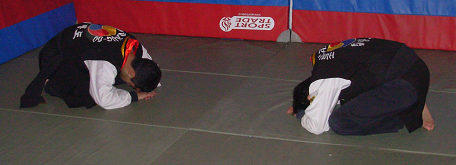
\includegraphics[width=0.5\textwidth]{images/Lucha_de_Piso/01_saludo.png}
	\caption{Saludo Budista Tradicional}
	\label{fig:saludo_budista_lp}
\end{figure}

\subsection*{Paso 2: Saludo Occidental Modificado}

Después del saludo budista, los practicantes pueden realizar un saludo occidental modificado, que es un gesto de cortesía occidental con un toque marcial. En este saludo, la mano izquierda se coloca debajo del brazo derecho extendido hacia adelante. Esta posición muestra respeto y preparación para el combate. Se ilustra en la Figura \ref{fig:saludo_occidental_lp}.

\begin{figure}[h]
	\centering
	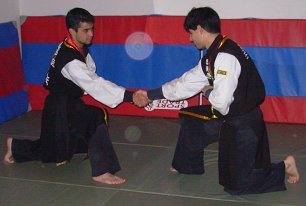
\includegraphics[width=0.5\textwidth]{images/Lucha_de_Piso/02_saludo_mano.png}
	\caption{Saludo Occidental Modificado}
	\label{fig:saludo_occidental_lp}
\end{figure}

\subsection*{Paso 3: Posición Inicial}

Una vez completados los saludos, los practicantes adoptan una posición inicial que varía según el estilo de lucha de piso. La posición inicial es fundamental para mantener el equilibrio y la preparación para cualquier movimiento. Se ilustra en la Figura \ref{fig:posicion_inicial_lp}.

\begin{figure}[h]
	\centering
	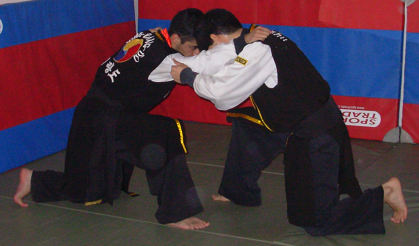
\includegraphics[width=0.5\textwidth]{images/Lucha_de_Piso/03_posicion_inicial.png}
	\caption{Posición Inicial}
	\label{fig:posicion_inicial_lp}
\end{figure}

Estos pasos iniciales establecen un ambiente de respeto y concentración, y preparan a los practicantes para la acción en la lucha de piso. Desde esta posición inicial, comienza la exploración de técnicas y estrategias esenciales en este emocionante aspecto de las artes marciales.


Es fundamental que los participantes comprendan y respeten estas reglas para garantizar un ambiente seguro y respetuoso durante la práctica de la lucha de piso escolar.

\subsection{Técnicas básicas de inmovilización}

¡Comencemos a explorar las técnicas básicas de inmovilización en la lucha de piso y a desarrollar tus habilidades en esta emocionante disciplina de las artes marciales!


\begin{enumerate}
	\item \textbf{Inmovilización Lateral:}

	\begin{itemize}
		\item Posición Inicial: En la Montada en Posición Crucifijo, un competidor se encuentra encima de su oponente, utilizando su propio cuerpo para presionar el pecho del oponente.

		\item Orientación Corporal: Quien está arriba adopta la posición boca arriba, mientras que el oponente está posicionado boca abajo en el suelo. Esta disposición inicial crea una ventaja estratégica para el luchador en la parte superior.

		\item Posición Perpendicular: La característica distintiva de esta técnica es que el practicante que está arriba se coloca de manera perpendicular al cuerpo del oponente. Esto significa que su torso atraviesa el torso del oponente en un ángulo de 90 grados, lo que le proporciona un control efectivo. Ver \ref{fig:posicion_lateral_frontal_lp}

		\item Rodilla bajo el Brazo: Además, quien está arriba posiciona una de sus rodillas debajo del brazo del oponente que está abajo. Esta táctica bloquea el movimiento del brazo del oponente y restringe sus opciones de defensa. Ver \ref{fig:posicion_lateral_lateral_lp}
	\end{itemize}

	% Mostrar una secuencia a 2 fotos
	\begin{figure}[h]
		\centering
		\begin{minipage}{0.45\textwidth}
			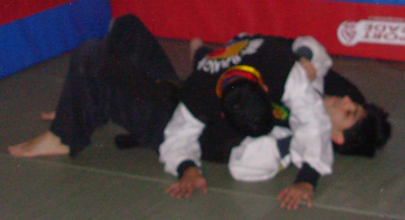
\includegraphics[width=\linewidth]{images/Lucha_de_Piso/04_posicion_lateral_a.png}
			\caption{Inmovilización lateral vista frontal}
			\label{fig:posicion_lateral_frontal_lp}
		\end{minipage}
		\hfill
		\begin{minipage}{0.45\textwidth}
			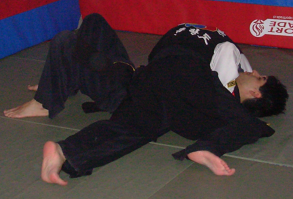
\includegraphics[width=\linewidth]{images/Lucha_de_Piso/05_posicion_lateral_b.png}
			\caption{Inmovilización lateral vista lateral}
			\label{fig:posicion_lateral_lateral_lp}
		\end{minipage}
		\hfill
	\end{figure}

	\item \textbf{Inmovilización de Pulpo:} El "Control del Pulpo" es una técnica de inmovilización en HwaRangDo que guarda similitudes con la anteriormente mencionada. La diferencia principal radica en que el oponente se encuentra sentado, ubicado cerca del hombro del practicante que ejecuta la técnica. A continuación, se detalla esta técnica: Ver \ref{fig:posicion_lateral_pulpo_lp}.

	\begin{itemize}
		\item Posición Inicial: El oponente se encuentra sentado, con su ubicación cercana al hombro del practicante que realiza la técnica.
		\item Abrazo de Brazos: Quien ejecuta la técnica rodea ambos brazos del oponente por detrás de su cabeza. Existen variantes en las que el practicante puede optar por cerrar la posición sujetando su propia corva o el cinturón del uniforme del oponente.
		\item Presión en el Pecho: El cuerpo del practicante que está arriba aplica presión sobre el pecho del oponente, restringiendo su capacidad de movimiento.
		\item Posición de las Piernas: Para mantener un control sólido, las piernas del practicante deben estar separadas y paralelas al suelo, asumiendo una forma abstracta que recuerda la de un pulpo.
	\end{itemize}

	\begin{figure}[h]
		\centering
		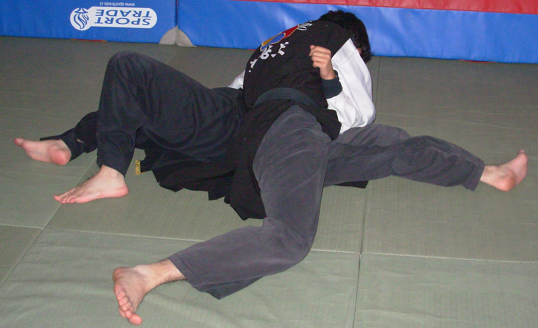
\includegraphics[width=0.5\textwidth]{images/Lucha_de_Piso/06_posicion_lateral_pulpo.png}
		\caption{Inmovilización de pulpo}
		\label{fig:posicion_lateral_pulpo_lp}
	\end{figure}


	\item \textbf{Inmovilización a una pierna:} En esta técnica de inmovilización, el ejecutor se coloca de manera perpendicular con respecto al oponente, quien puede estar boca arriba (Figura \ref{fig:inmovilizacion_una_pierna_frontal_lp}) o boca abajo en el suelo (Ver Figura \ref{fig:inmovilizacion_una_pierna_lateral_lp}). Los pasos clave son los siguientes:

	\begin{itemize}
		\item El ejecutor coloca uno de sus brazos por detrás de la nuca del oponente.
		\item El otro brazo se desliza por debajo de ambos muslos del oponente.
		\item Ambas manos del ejecutor intentan unirse para completar la inmovilización.
	\end{itemize}

	% Mostrar una secuencia a 2 fotos
	\begin{figure}[h]
		\centering
		\begin{minipage}{0.45\textwidth}
			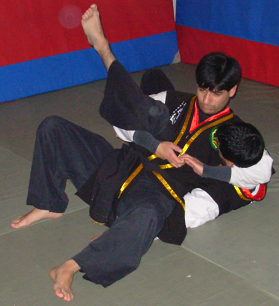
\includegraphics[width=\linewidth]{images/Lucha_de_Piso/07_inmovilizacion_a_una_pierna_frontal.png}
			\caption{Posición de inmovilización a una pierna boca arriba}
			\label{fig:inmovilizacion_una_pierna_frontal_lp}
		\end{minipage}
		\hfill
		\begin{minipage}{0.45\textwidth}
			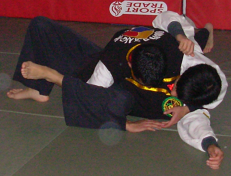
\includegraphics[width=\linewidth]{images/Lucha_de_Piso/08_inmovilizacion_a_una_pierna_lateral.png}
			\caption{Posición de inmovilización a una pierna boca abajo}
			\label{fig:inmovilizacion_una_pierna_lateral_lp}
		\end{minipage}
		\hfill
	\end{figure}

	\item \textbf{Inmovilización a dos piernas:} En esta técnica de inmovilización, el ejecutor se coloca de manera perpendicular con respecto al oponente, quien puede estar boca arriba (Figura \ref{fig:inmovilizacion_dos_piernas_frontal_lp}) o boca abajo en el suelo (Ver Figura \ref{fig:inmovilizacion_dos_piernas_lateral_lp}). Los pasos clave son los siguientes:

	\begin{itemize}
		\item El ejecutor coloca uno de sus brazos por detrás de la nuca del oponente.
		\item El otro brazo se desliza por debajo del muslo del oponente.
		\item Ambas manos del ejecutor intentan unirse para completar la inmovilización.
	\end{itemize}


	% Mostrar una secuencia a 2 fotos
	\begin{figure}[h]
		\centering
		\begin{minipage}{0.45\textwidth}
			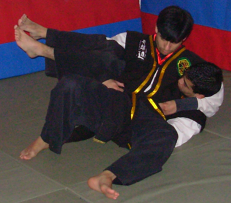
\includegraphics[width=\linewidth]{images/Lucha_de_Piso/09_inmovilizacion_a_una_pierna_lateral.png}
			\caption{Posición de retención lateral vista frontal}
			\label{fig:inmovilizacion_dos_piernas_frontal_lp}
		\end{minipage}
		\hfill
		\begin{minipage}{0.45\textwidth}
			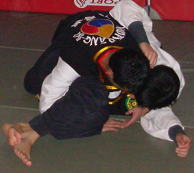
\includegraphics[width=\linewidth]{images/Lucha_de_Piso/10_inmovilizacion_a_una_pierna_lateral.png}
			\caption{Inmovilización lateral vista lateral}
			\label{fig:inmovilizacion_dos_piernas_lateral_lp}
		\end{minipage}
		\hfill
	\end{figure}



	\item \textbf{Inmovilización abrazo de cintura:} En esta técnica de inmovilización, el ejecutor abraza al oponente por la espalda a la altura de la cintura. Los pasos clave son los siguientes: Ver \ref{fig:posicion_abrazo_cintura}.

	\begin{itemize}
		\item El ejecutor rodea al oponente por la cintura con sus brazos, asegurando un agarre sólido.
		\item Luego, intenta bajar o acercar su propia cadera al suelo lo más posible.
		\item El pie que está más cerca del oponente se abre, y la parte interna de este pie queda tocando el suelo.
	\end{itemize}

	Esta técnica genera una especie de ''peso muerto`` que dificulta al oponente escapar, ya que el ejecutor tiene un control efectivo sobre su cintura y ha establecido una base sólida en el suelo.

	\begin{figure}[h]
		\centering
		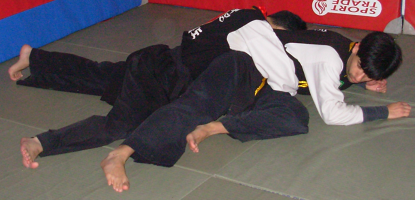
\includegraphics[width=0.5\textwidth]{images/Lucha_de_Piso/11_inmovilizacion_abrazo_cintura.png}
		\caption{Inmovilización de cintura}
		\label{fig:posicion_abrazo_cintura}
	\end{figure}

	\item \textbf{Inmovilización de montada} La inmovilización de montada en HwaRangDo se asemeja a la posición de un jinete montando a caballo. Los pasos clave de esta técnica son los siguientes: . Ver \ref{fig:posicion_montada}.

	\begin{itemize}
		\item \textbf{Posición del Ejecutor:} El practicante se coloca sobre el oponente, sentándose sobre su torso. Esta posición proporciona un control total sobre el oponente.
		\item \textbf{Unión del Pecho:} El ejecutor acerca su pecho al rostro del oponente, minimizando la capacidad de movimiento de este último.
		\item \textbf{Brazos detrás de la Cabeza:} Los brazos del practicante se juntan detrás de la cabeza del oponente. Esta posición no solo limita la capacidad de defensa del oponente, sino que también prepara el terreno para posibles estrangulamientos y sumisiones.
	\end{itemize}

	La inmovilización de montada es una posición de control fundamental en el Jiu-Jitsu, que permite al practicante dominar y mantener al oponente en el suelo mientras busca oportunidades para someterlo o avanzar hacia técnicas adicionales.

	\begin{figure}[h]
		\centering
		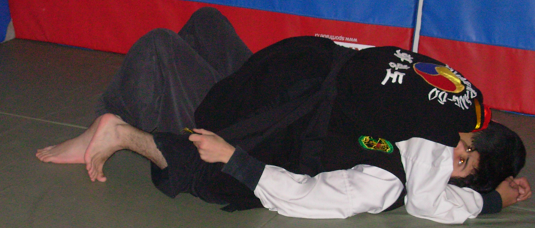
\includegraphics[width=0.5\textwidth]{images/Lucha_de_Piso/12_inmovilizacion_montado.png}
		\caption{Inmovilización de montada}
		\label{fig:posicion_montada}
	\end{figure}

	\item \textbf{Inmovilización de tijeras:}     La "Posición de Tijeras" es una técnica en HwaRangDo en la cual el ejecutor utiliza sus piernas para abrazar al oponente. Ver \ref{fig:posicion_tijeras}.

	En esta posición:

	\begin{itemize}
		\item El practicante entrelaza sus piernas alrededor del cuerpo del oponente.
		\item Esta técnica crea un bloqueo efectivo y limita la capacidad de movimiento del oponente.
		\item La "Posición de Tijeras" puede ser utilizada como una estrategia de control en el suelo o como preparación para aplicar sumisiones adicionales.
	\end{itemize}

	La ''Posición de Tijeras`` es una herramienta importante en el arsenal de técnicas de control y sumisión de HwaRangDo, permitiendo al practicante mantener a raya al oponente y buscar oportunidades para asegurar la victoria. \footnote{Para obtener la victoria, el que abraza con las piernas, debe estar sobre la espalda del oponente sin estrangularlo} . Ver \ref{fig:posicion_tijeras}.

	\begin{figure}[h]
		\centering
		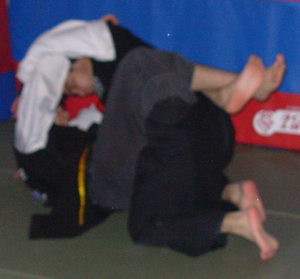
\includegraphics[width=0.5\textwidth]{images/Lucha_de_Piso/13_inmovilizacion_tijeras.png}
		\caption{Inmovilización de Tijeras}
		\label{fig:posicion_tijeras}
	\end{figure}
\end{enumerate}


\subsection{Técnicas avanzadas de inmovilización}

\begin{enumerate}

	\item \textbf{Inmovilización de tronco:} Explicación posición de Inmovilización de tronco. Ver \ref{fig:inmovilizacion_tronco_1}. Ver \ref{fig:inmovilizacion_tronco_2}.

	\begin{figure}[h]
		\centering
		\begin{minipage}{0.45\textwidth}
			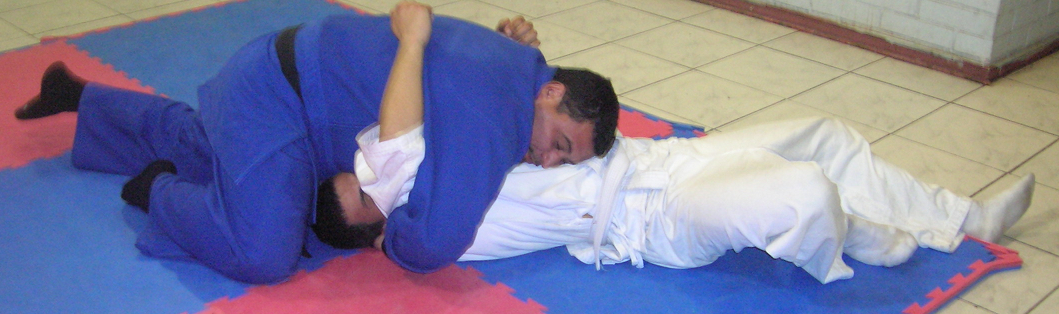
\includegraphics[width=\linewidth]{images/Lucha_de_Piso/14_inmovilizacion_pecho.png}
			\caption{Posición de retención lateral vista frontal}
			\label{fig:inmovilizacion_tronco_1}
		\end{minipage}
		\hfill
		\begin{minipage}{0.45\textwidth}
			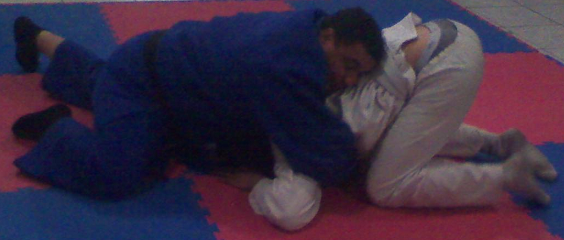
\includegraphics[width=\linewidth]{images/Lucha_de_Piso/15_inmovilizacion_pecho.png}
			\caption{Inmovilización lateral vista lateral}
			\label{fig:inmovilizacion_tronco_2}
		\end{minipage}
		\hfill
	\end{figure}


	\begin{figure}[h]
		\centering
		\begin{minipage}{0.45\textwidth}
			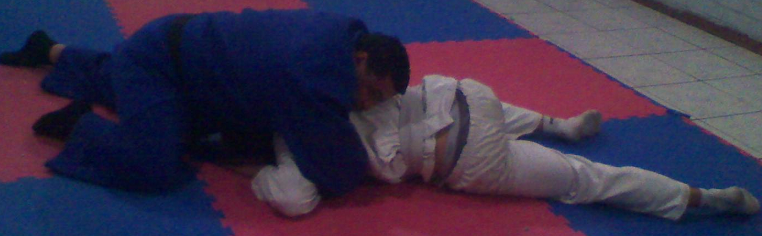
\includegraphics[width=\linewidth]{images/Lucha_de_Piso/16_inmovilizacion_pecho.png}
			\caption{Posición de retención lateral vista frontal}
			\label{fig:inmovilizacion_tronco_3}
		\end{minipage}
		\hfill
		\begin{minipage}{0.45\textwidth}
			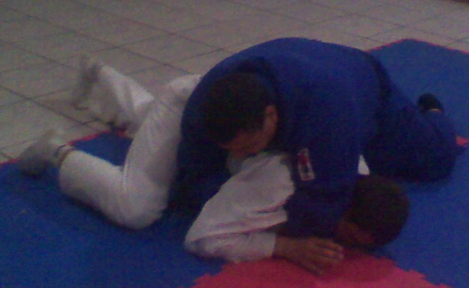
\includegraphics[width=\linewidth]{images/Lucha_de_Piso/17_inmovilizacion_pecho.png}
			\caption{Inmovilización lateral vista lateral}
			\label{fig:inmovilizacion_tronco_4}
		\end{minipage}
		\hfill
	\end{figure}


	\item \textbf{Inmovilización de Pulpo con tomada de brazo:} Explicación posición de Inmovilización de tronco. Ver \ref{fig:inmovilizacion_tronco_1}. Ver \ref{fig:inmovilizacion_tronco_2}.
	\begin{figure}[h]
		\centering
		\begin{minipage}{0.45\textwidth}
			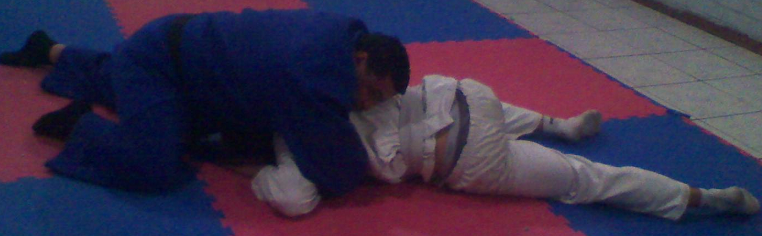
\includegraphics[width=\linewidth]{images/Lucha_de_Piso/16_inmovilizacion_pecho.png}
			\caption{Posición de retención lateral vista frontal}
			\label{fig:inmovilizacion_pulpo_arriba_tomada_de brazo}
		\end{minipage}
		\hfill
	\end{figure}

	\item \textbf{Inmovilización de Pulpo con tomada de brazo doble:} Explicación posición de Inmovilización de tronco. Ver \ref{fig:inmovilizacion_tronco_1}. Ver \ref{fig:inmovilizacion_tronco_2}.
	\begin{figure}[h]
		\centering
		\begin{minipage}{0.45\textwidth}
			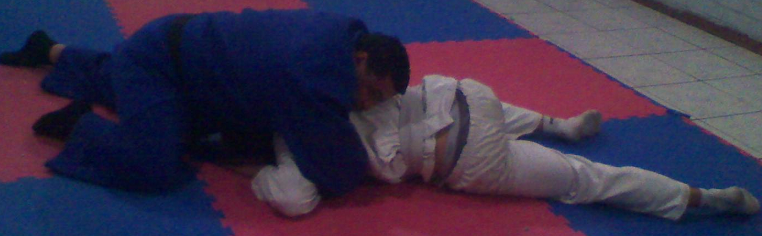
\includegraphics[width=\linewidth]{images/Lucha_de_Piso/16_inmovilizacion_pecho.png}
			\caption{Posición de retención lateral vista frontal}
			\label{fig:inmovilizacion_pulpo_arriba_tomada_de brazo_doble}
		\end{minipage}
		\hfill
	\end{figure}

	\item \textbf{Inmovilización de espalda:} Explicación posición de Inmovilización de tronco. Ver \ref{fig:inmovilizacion_tronco_1}. Ver \ref{fig:inmovilizacion_de_espalda}.
	\begin{figure}[h]
		\centering
		\begin{minipage}{0.45\textwidth}
			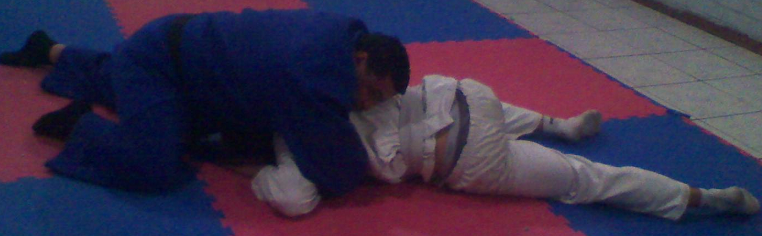
\includegraphics[width=\linewidth]{images/Lucha_de_Piso/16_inmovilizacion_pecho.png}
			\caption{Posición de retención de espalda}
			\label{fig:inmovilizacion_de_espalda}
		\end{minipage}
		\hfill
	\end{figure}

\end{enumerate}
